%4. Problem space (Prototype, test setups, existing software)
\chapter{Understanding the Problem Space}
\label{chap:understanding-the-problem-space}
In order to provide a satisfying solution to the problem at hand, the problem itself and the environment it occurs in must be researched. This chapter aims to explore and examine the problem space, resulting in a set of artefacts (namely a domain model and a set of requirements) that aid in understanding the context and designing an appropriate solution. First, a prototypical network proxy is designed and implemented in section \ref{sec:prototypical-implementation} to get an understanding of the problems and challenges involved in designing, implementing and using such software. Based on these experiences, interviews with experts in penetration testing are conducted and evaluated in section \ref{sec:interviews} to get a proper understanding of their everyday work and resulting problems. Lastly, existing software that aims to intercept communication for various scenarios and technologies is examined in section \ref{sec:analysis-existing-software}, compared to each other and their usefulness for the problem-specific scenarios is assessed. %TODO: Rewrite & update

\section{Prototypical Implementation}
\label{sec:prototypical-implementation}
The prototype was designed to be used in three different scenarios, each taking place in a different context. The goal of this section was to implement a prototype that could be used as a proxy to intercept communication between an \ac{IoT} device and its cloud service as shown in figure \ref{fig:network-communication-diagrams}. It was developed incrementally so individual components could be derived from requirements, designed, implemented and evaluated in fixed sprints.

\begin{figure}%
    \centering
    \subfloat[\centering Regular communication between an \ac{IoT} device and a cloud service.]{{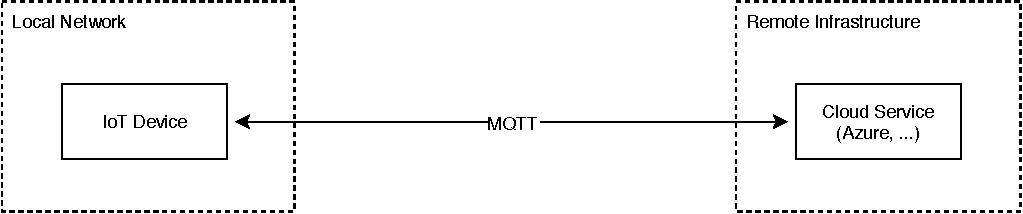
\includegraphics[width=10cm]{img/ch04/Setup - 1 Regular.pdf} }}%
    \qquad
    \subfloat[\centering Communication intercepted by a \ac{MITM} proxy.]{{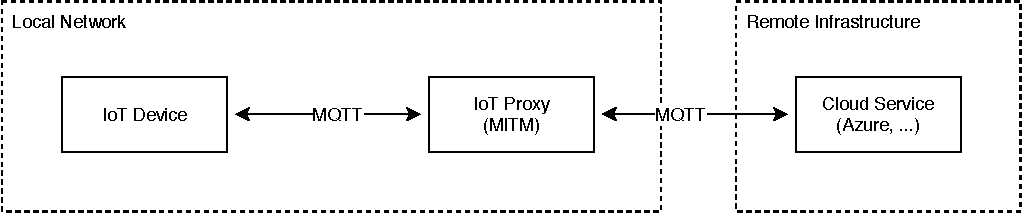
\includegraphics[width=10cm]{img/ch04/Setup - 2 Pentesting.pdf} }}%
    \caption{Installing a \ac{MITM} proxy to intercept network communication for penetration testing.}%
    \label{fig:network-communication-diagrams}%
\end{figure}

\subsection{Example Scenarios}
\label{sec:example-scenarios}
The following scenarios describe hypothetical configurations of \ac{IoT}/\ac{IIoT} devices that should be tested with the prototype and vary in both technical and logical complexity as well as in closeness to reality:

\subsubsection{Scenario \#1: Legacy \ac{ICS} Application}
\label{par:scenario-1}
In this \ac{IIoT} scenario, a \ac{HMI} (e.g. \emph{Siemens KTP400 Basic}) sends commands to and receives data from a \ac{PLC} (e.g. \emph{Siemens S7-1200}) using Modbus \ac{TCP} (depicted in figure \ref{fig:arch-ics}). The \ac{PLC} continually counts up a value up to 100 and begins anew at zero while the \ac{HMI} displays the current value and provides a button that, upon being pressed by a user, resets the current value to zero. \\
In this scenario, attackers could perform a variety of attacks on the system by intercepting and manipulating network traffic, for example:
\begin{figure}[h]
    \centering
    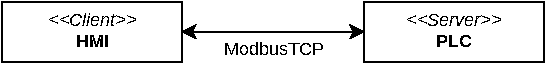
\includegraphics{img/ch04/Scenario_ICS.pdf}
    \captionof{figure}{?} %TODO: Describe
    \label{fig:arch-ics}
\end{figure}
\begin{itemize}
    \item By dropping messages sent from the \ac{PLC} to the \ac{HMI}, the application may appear unresponsive as new data is not displayed on the \ac{HMI}. In production environments, this could lead to dangerous situations as sensor readings that indicate harmful environmental conditions would not be presented to supervising personnel.
    \item When dropping messages sent from the \ac{HMI} to the \ac{PLC}, control commands can be suppressed. This attack can result in catastrophic situations when emergency shutdowns issued by supervising personnel are not registered by the affected machines.
\end{itemize}
Although this scenario involves a rather simple process, it depicts a realistic communication configuration. It focusses on the use of a legacy transport protocol. Due to the rather simple nature of the Modbus \ac{TCP} protocol, intercepting and manipulating communication is expected to be trivial. %TODO: Add diagram?
%https://support.industry.siemens.com/tf//WW/en/posts/s7-1500-communication-and-modbus-tcp-on-hmi/144092?page=0&pageSize=10
%https://support.industry.siemens.com/cs/pd/379924?pdti=td&dl=en&lc=en-DK

\subsubsection{Scenario \#2: \ac{IoT} Cloud Application}
\label{par:scenario-2} As shown in figure \ref{fig:arch-smart-home}, this \ac{IoT} smart home scenario utilizes two local \ac{IoT} devices that are integrated into a cloud environment such as the \ac{AWS} \ac{IoT} platform: a thermometer and an \ac{A/C} unit. Both devices connect to the cloud platform, authorize themselves at a \ac{REST} interface via \ac{HTTP} and upgrade their \ac{HTTP}-connection to \ac{WS} streams upon successful authorization. They eventually communicate to a remote \ac{MQTT} broker by tunnelling \ac{MQTT} packets over the \ac{WS} stream. At this stage, the thermometer publishes temperature readings to an \ac{MQTT} topic while the \ac{A/C} unit subscribes to the same topic and adjusts its operation depending on the incoming temperature readings. \\
This distributed communication setup introduces a set of possible attacks that could be performed when attackers \emph{impersonated} client-devices or the remote server:
\begin{figure}[h]
    \centering
    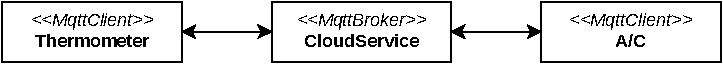
\includegraphics{img/ch04/Scenario_SmartHome.pdf}
    \captionof{figure}{?} %TODO: Describe
    \label{fig:arch-smart-home}
\end{figure}
\begin{itemize}
    \item Impersonating the thermometer, attackers could send incorrect temperature data and effectively control the \ac{A/C} unit. When sending low temperature readings while the environment temperature is high, the \ac{A/C} unit would stop running. Conversely, when high temperature readings are sent while the environment temperature is low, the \ac{A/C} unit would run, and thus further cool down the environment.
    \item Attackers that impersonate the remote server could drop or manipulate incoming publish packets, thus altering whether and/or what information is relayed other connected devices. For example, temperature readings that indicate a high environment temperature that would lead to the \ac{A/C} unit to be powered up could be rewritten in such a way that the transmitted temperature value is considered to indicate a low environment temperature, thus preventing the \ac{A/C} unit from running automatically.
\end{itemize}

\begin{figure}[h]
    \centering
    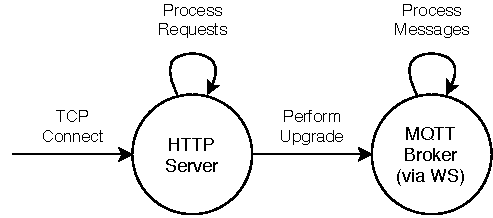
\includegraphics[width=6cm]{img/ch04/Statemachine 2.pdf}
    \captionof{figure}{State machine of \ac{AWS} \ac{IoT} communication}
    \label{fig:aws-statemachine}
\end{figure}
This scenario makes use of three communication protocols, uses these protocols dependent on the state of authentication and even tunnels one protocol through another one. Therefore the proxy application has to implement a state-machine (as seen in figure \ref{fig:aws-statemachine}) and testing communication in this scenario is expected to be more complex than the first one. Also, since this scenario makes use of the \ac{AWS} \ac{IoT} infrastructure, special care must be taken to ensure that authentication is properly relayed to the cloud servers.

% Reference: https://aws.amazon.com/blogs/aws/aws-iot-cloud-services-for-connected-devices/

\subsubsection{Scenario \#3: Water Treatment Plant}
\label{par:scenario-3}Similar to scenario \#2, this scenario makes use of \ac{MQTT} for transporting messages. However, the scenario takes place in an \ac{ICS} context of critical infrastructure.

\begin{figure}[h!]
    \centering
    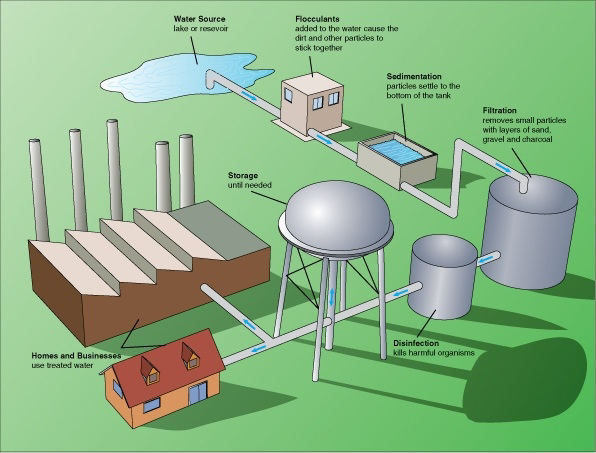
\includegraphics[width=12cm]{img/ch04/watertreatmentplant.png}
    \caption[Illustration of a typical drinking water treatment process. (by the CK-12 Foundation)]{Illustration of a typical drinking water treatment process. (by the CK-12 Foundation)\protect\footnotemark}
    \label{fig:water-treatment}
\end{figure}
\footnotetext{https://en.wikipedia.org/wiki/File:Illustration\_of\_a\_typical\_drinking\_water\_treatment\_process.png}

As shown in figure \ref{fig:water-treatment}, there are multiple steps involved in treating water for drinking. The scenario represents these steps as separate stations (\enquote{source}, \enquote{flocculants}, \enquote{sedimentation}, \enquote{filtration}, \enquote{disinfection} and \enquote{storage}) that act as \ac{MQTT} clients. Each station receives water into an input tank, processes water from its input tank in a specified rate and flushes processed water into an output tank. Similar to how threads can suffer from starvation in a multithreading environment, these stations can either \enquote{run dry} when their input tank is empty or overflow when either tank is filled beyond their capacity. In this scenario, stations will only process water from their input tanks if their output tank provides sufficient available capacity.\\
Similar to scenario \#2, attackers could perform a series of attacks in this scenario:
\begin{itemize}
    \item Without intercepting any communication, attackers could cyclically overwrite water levels of either input and output tanks to stop stations and bring processing to a halt. For example, when attackers overwrite the \enquote{storage} station's input tank level to indicate exhausted capacities, the \enquote{disinfection} station would fill its output tank and eventually stop processing water. This would cause the \enquote{disinfection} station's input tank to fill up and lead to the \enquote{filtration} station's output tank to fill up. Ultimately, the water treatment plant would halt.
    \item When any station publishes data about its tanks' levels indicating full or empty capacities, attackers could intercept those messages and change them to either indicate the opposite (change tank levels indicating \emph{full} capacities to levels indicating \emph{empty} capacity) or some arbitrary level information. This could lead to either pumping water from empty tanks, potentially damaging the pumps, or to overfilling tanks, leading to leaking excess water and potentially damaging further equipment.
    \item Attackers that intercept messages between the stations and the broker can collect and analyse them and try to draw conclusions about the use and activity of the system. This may allow attackers to identify patterns that show when the plant is operating at high capacities, maximizing the effect of attacks against the plant.
\end{itemize}
\begin{figure}[h!]
    \centering
    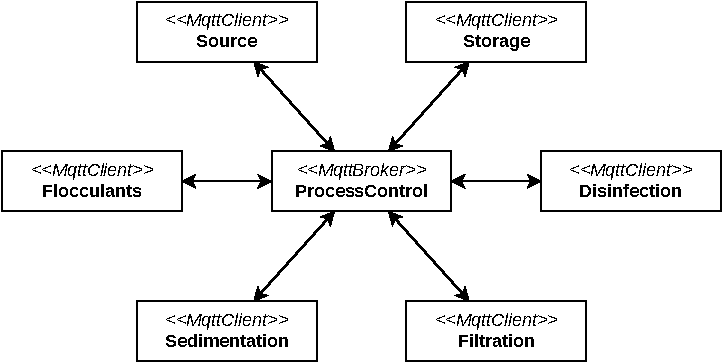
\includegraphics[width=10cm]{img/ch04/Scenario_WTP.pdf}
    \caption[?]{?}
    \label{fig:arch-water-treatment}
\end{figure}
This scenario greatly simplifies drinking water treatment by reducing the process to the producer-consumer problem known from multithreading. A more realistic representation of drinking water treatment plants would take further details, such as chemicals used in disinfection, into account.\\ %TODO: Cite!
This scenario involves only \ac{MQTT} as a transport protocol but, as can be seen in figure \ref{fig:arch-water-treatment}, it requires six \ac{MQTT} clients to run simultaneously.

\subsubsection{Derived Use-Cases} Summarizing the scenarios detailed above, a number of high-level use-cases can be derived from them (shown in \ref{fig:use-cases-scenarios}). The actors are the \emph{attacker} that intends to interact with the system in a potentially malicious way and the \emph{server} and \emph{client} that use the system for transportation of messages. The following use-cases are found in the aforementioned scenarios:

\begin{figure}[h]
    \centering
    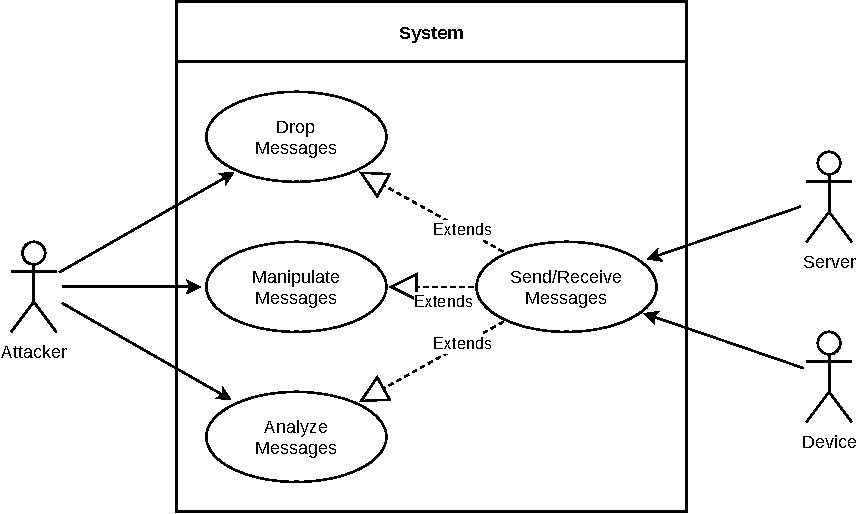
\includegraphics[width=14cm]{img/ch04/UseCases_Scenarios.pdf}
    \captionof{figure}{High-level use-cases of a proxy in a generic \ac{IoT}/\ac{ICS} environment.}
    \label{fig:use-cases-scenarios}
\end{figure}


\begin{itemize}
    \item \textbf{Send/Receive Messages:} The server and client send and receive messages to communicate with each other. This interaction does not require interaction with the attacker.
    \item \textbf{Drop Messages:} The attacker discards incoming or outgoing messages by not relaying them to the intended target. This can cause loss of control in the application that this communication takes place in.
    \item \textbf{Manipulate Messages:} Incoming or outgoing messages can be changed by an attacker, altering various properties such as \ac{QoS} (for \ac{MQTT} messages), host (for \ac{HTTP} requests) or the payload of a message (e.g. the content of an \ac{HTTP} response).
    \item \textbf{Analyse Messages:} Attackers can collect and analyse passively without altering them, allowing them to deduce information about the behaviour of the affected system and potentially its user(s).
\end{itemize}

\subsection{Requirements}
To be able to operate in all of the aforementioned scenarios, the prototype had to implement a set of functional requirements:

%F1
\begin{center}

    \begin{tabular}{|p{1cm}|p{12cm}|}
        \hline
        \textbf{F1} & \textbf{Protocols}                                                                                                                                                                                    \\ \hline
        \multicolumn{2}{|p{12cm}|}{The software must implement parsing/crafting messages/packets of the communication protocols: \ac{HTTP}\footnotemark, \ac{WS}, \ac{MQTT} and Modbus \ac{TCP}.}                           \\ \hline
        \multicolumn{2}{|p{12cm}|}{\textbf{Fit criterion:} The software must implement and support the \ac{HTTP}, \ac{WS} and \ac{MQTT} protocols so messages of those protocols can be further processed by the software.} \\ \hline
    \end{tabular}
\end{center}
\footnotetext{\ac{HTTPS} was deemed relevant as the prototype as of an academic nature and the addition of \ac{SSL} introduced further complexity.}
%F2
\begin{center}

    \begin{tabular}{|p{1cm}|p{12cm}|}
        \hline
        \textbf{F2} & \textbf{Network Stacks}                                                                                                                                                                                                                                                                                                      \\ \hline
        \multicolumn{2}{|p{12cm}|}{The software must be able to parse protocols that are tunnelled through other protocols (\enquote{\emph{stacked}}). It must provide an interface to the user where they can specify which communication protocols are used and whether and how they are stacked (further referred to as \emph{network stack}).} \\ \hline
        \multicolumn{2}{|p{12cm}|}{\textbf{Fit criterion:} The software processes a configuration file that lets users specify which protocols to be used and whether/how they are stacked.}                                                                                                                                                       \\ \hline
    \end{tabular}
\end{center}
%F3
\begin{center}

    \begin{tabular}{|p{1cm}|p{12cm}|}
        \hline
        \textbf{F3} & \textbf{State-Machines}                                                                                                                                                                                                                                                                                                                                 \\ \hline
        \multicolumn{2}{|p{12cm}|}{The software must be able to switch network stacks and scripts for processing dependent on configurable \emph{states} and \emph{transitions} between them. It must provide an interface for the user to specify when to switch to using another network stack, represented using \acp{FSM} and rule sets for transmission between states.} \\ \hline
        \multicolumn{2}{|p{12cm}|}{\textbf{Fit criterion:} The software processes a configuration file that lets users specify when to switch between network stacks.}                                                                                                                                                                                                        \\ \hline
    \end{tabular}
\end{center}
%F4
\begin{center}

    \begin{tabular}{|p{1cm}|p{12cm}|}
        \hline
        \textbf{F4} & \textbf{Integration}                                                                                                                                    \\ \hline
        \multicolumn{2}{|p{12cm}|}{The software shall provide interfaces for integration of third-party software.}                                                            \\ \hline
        \multicolumn{2}{|p{12cm}|}{\textbf{Fit criterion:} The software implements interfaces that allow sending packets to other applications such as \enquote{Burp Suite}.} \\ \hline
    \end{tabular}
\end{center}
%F5
\begin{center}

    \begin{tabular}{|p{1cm}|p{12cm}|}
        \hline
        \textbf{F5} & \textbf{Scripting}                                                                                                     \\ \hline
        \multicolumn{2}{|p{12cm}|}{The software shall provide scripting capabilities for automated manipulation and discarding of messages.} \\ \hline
        \multicolumn{2}{|p{12cm}|}{\textbf{Fit criterion:} Users can define scripts that are executed on messages.}                          \\ \hline
    \end{tabular}
\end{center}
%F6
\begin{center}
    \begin{tabular}{|p{1cm}|p{12cm}|}
        \hline
        \textbf{F6} & \textbf{Logging}                                                                                       \\ \hline
        \multicolumn{2}{|p{12cm}|}{The software shall provide means for collecting and saving messages for future analysis.} \\ \hline
        \multicolumn{2}{|p{12cm}|}{\textbf{Fit criterion:}The software saves messages to a MySQL database.}                  \\ \hline
    \end{tabular}
\end{center}
The following non-functional requirements were defined:

%N1
\begin{center}
    \begin{tabular}{|p{1cm}|p{12cm}|}
        \hline
        \textbf{N1} & \textbf{Platform Compatibility}                                                                                                   \\ \hline
        \multicolumn{2}{|p{12cm}|}{In order to support a broad spectrum of target platforms, the software shall be implemented platform-independently.} \\ \hline
    \end{tabular}
\end{center}
%N2
\begin{center}
    \begin{tabular}{|p{1cm}|p{12cm}|}
        \hline
        \textbf{N2} & \textbf{Reusability}                                                                                                                  \\ \hline
        \multicolumn{2}{|p{12cm}|}{The software shall be reusable so it can be used in future tests that may feature new configurations of network stacks.} \\ \hline
    \end{tabular}
\end{center}
%N3
\begin{center}
    \begin{tabular}{|p{1cm}|p{12cm}|}
        \hline
        \textbf{N3} & \textbf{Open Source}                                                                                                                                 \\ \hline
        \multicolumn{2}{|p{12cm}|}{The software shall be available as open source software so programmers and members of the IT community may contribute to improving it.} \\ \hline
    \end{tabular}
\end{center}

Due to this implementation serving as a prototype and being of an academic nature, no specific constraints were defined. It was to be developed strictly ignoring aspects of usability and stability as it should not be used in production environments but in laboratories exclusively.

\subsection{Design}
\label{sec:prototype-design}
The prototype was designed to be fit for use in the second scenario as, regarding network communication, it was more complex than the other ones. Specifically, the second scenario demanded the implementation of a network stack and a state machine to switch between states.
Parsing protocols that were tunnelled through other protocols appeared to be a potentially challenging requirement which is why the focus on the design and implementation of this prototype was on the underlying management, processing and relaying of messages. In order to tackle it, a variation of the \emph{pipeline} (sometimes referred to \emph{pipes and filters}) design pattern was used (as shown in figure \ref{fig:design-pipes-and-filters}). It was designed to be used as follows:\par
\emph{Messages} originate from a listener, for example messages with raw byte payloads are received from a \ac{TCP} socket. These messages are sent to an initial \emph{pipe} to be processed \emph{down}.

\begin{figure}[h]
    \centering
    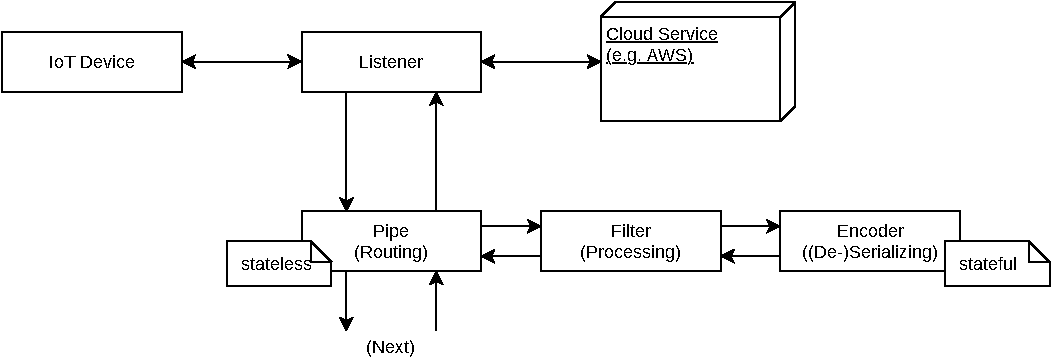
\includegraphics[width=14cm]{img/ch04/Architecture - Pipes and Filters4.pdf}
    \captionof{figure}{The variation of the \enquote{pipes and filters} design pattern used in the prototype.}
    \label{fig:design-pipes-and-filters}
\end{figure}
Pipes are bi-directional routers that represent processing-steps of pipelines and perform the following actions on messages that are processed through a pipeline:
\begin{enumerate}
    \item Pipes use optional \emph{encoders} to disassemble/de-serialize messages when processing them \emph{down} the pipeline and re-assemble/serialize them when they process messages \emph{up} the pipeline.
    \item Pipes can use \enquote{filters} to perform operations on messages such as replacing header values or manipulating payloads.
    \item They forward messages to the next pipe in its pipeline when processing messages down or to the previous pipe when processing messages back up.
\end{enumerate}
There are extensions to basic pipes such as:
\begin{itemize}
    \item \emph{EndPipes} are appended to the end of a pipeline and reverse the message processing direction so messages that were processed down are sent back up the pipeline to be processed up.
    \item \emph{ProcessingPipes} mandate encoders and filters to be used. These pipes are used to indicate that messages are not not only routed but also processed and encoded or decoded.
    \item \emph{IntegrationPipes} allow integration of other software into the pipeline. For example, penetration testing software such as Burp Suite could be integrated.
\end{itemize}

\begin{figure}[h!]
    \centering
    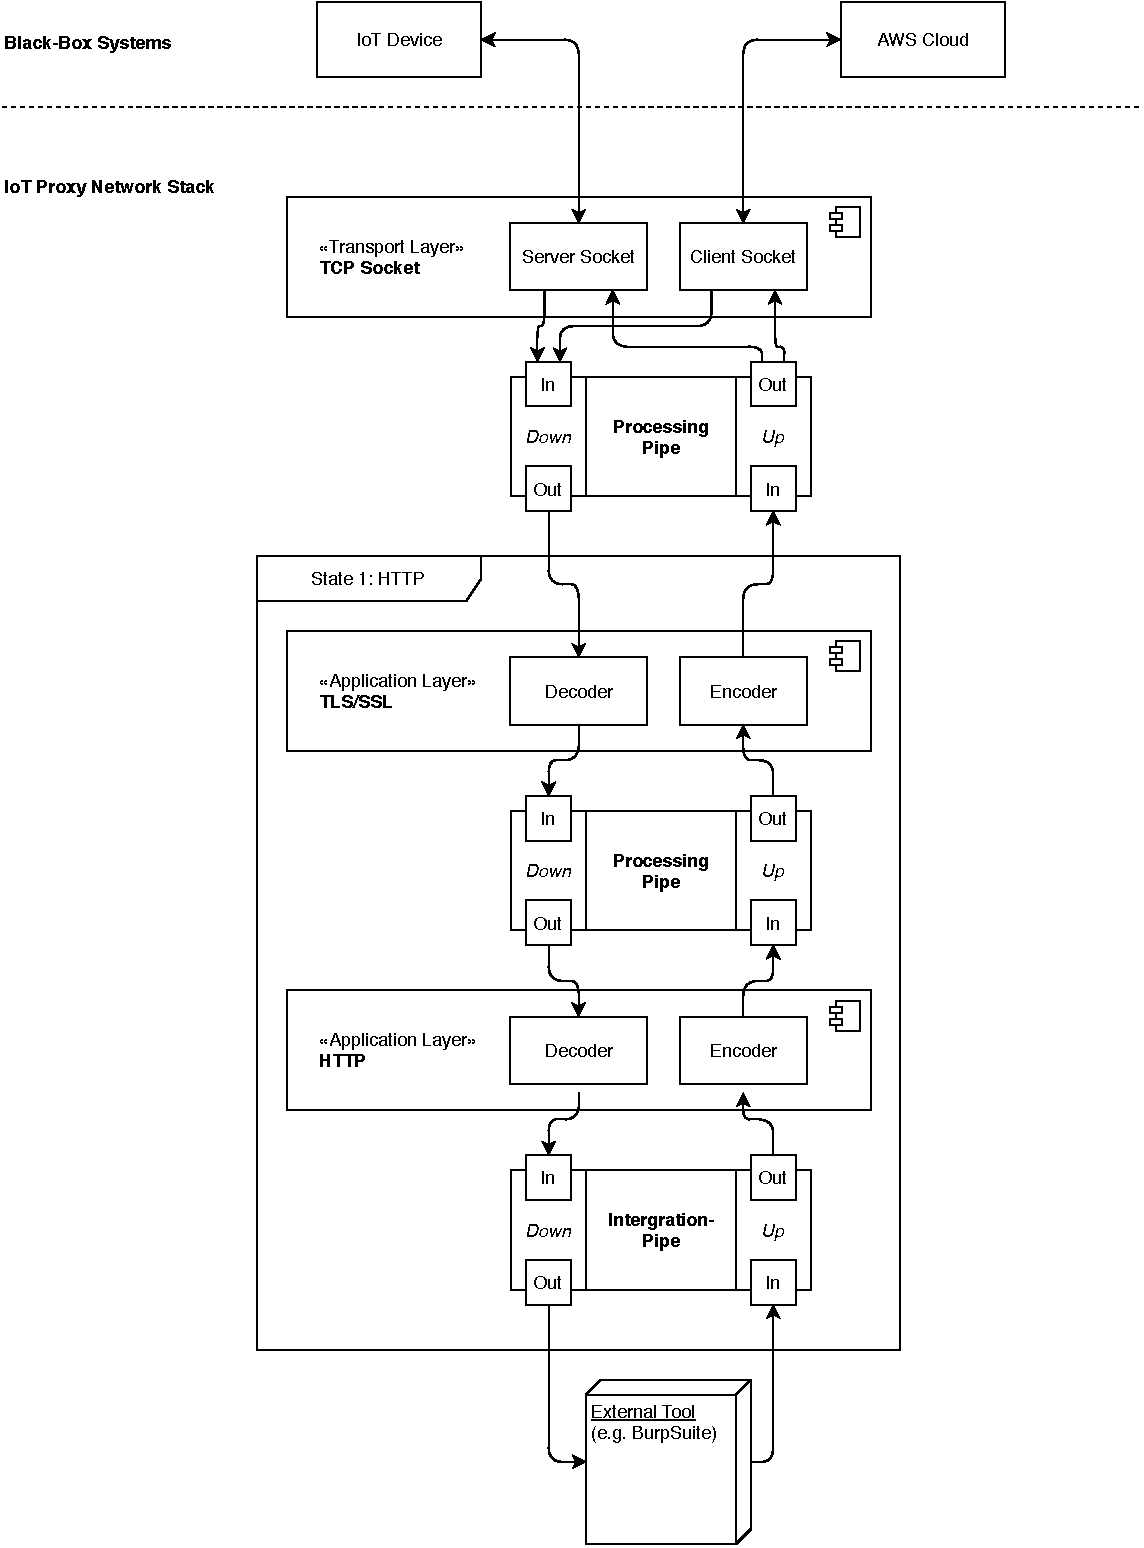
\includegraphics[width=14cm]{img/ch04/Architecture - PipesFilters 1.pdf}
    \captionof{figure}{\ac{AWS} \ac{IoT} Scenario - State 1: \ac{HTTP} Server}
    \label{fig:app-diag-pipesfilters-1}
\end{figure}
An exemplaric configuration of the pipeline design pattern envisioned for this prototype for use in the \ac{AWS} \ac{IoT} scenario is shown in figures \ref{fig:app-diag-pipesfilters-1} and \ref{fig:app-diag-pipesfilters-2}. These diagrams visualize how messages are processed \emph{down} and back \emph{up}.\\
Figure \ref{fig:app-diag-pipesfilters-1} shows the first state of the \ac{AWS} \ac{IoT} scenario that processes \ac{HTTP} communication. It features a TCP server socket that accepts incoming connection requests from an \ac{IoT} device and a client socket that is connected to the \ac{AWS} cloud. Since the communication to the \ac{AWS} cloud is \ac{TLS}-encrypted, it is first decrypted by a filter and then processed by a \ac{HTTP} filter. Then, the parsed \ac{HTTP} requests and responses are sent to external tools (e.g. BurpSuite). Once the end of the pipeline is reached, the messages are sent back up the pipeline, being encoded back into a form usable for the \ac{IoT} device or cloud server.\\
\begin{figure}[h!]
    \centering
    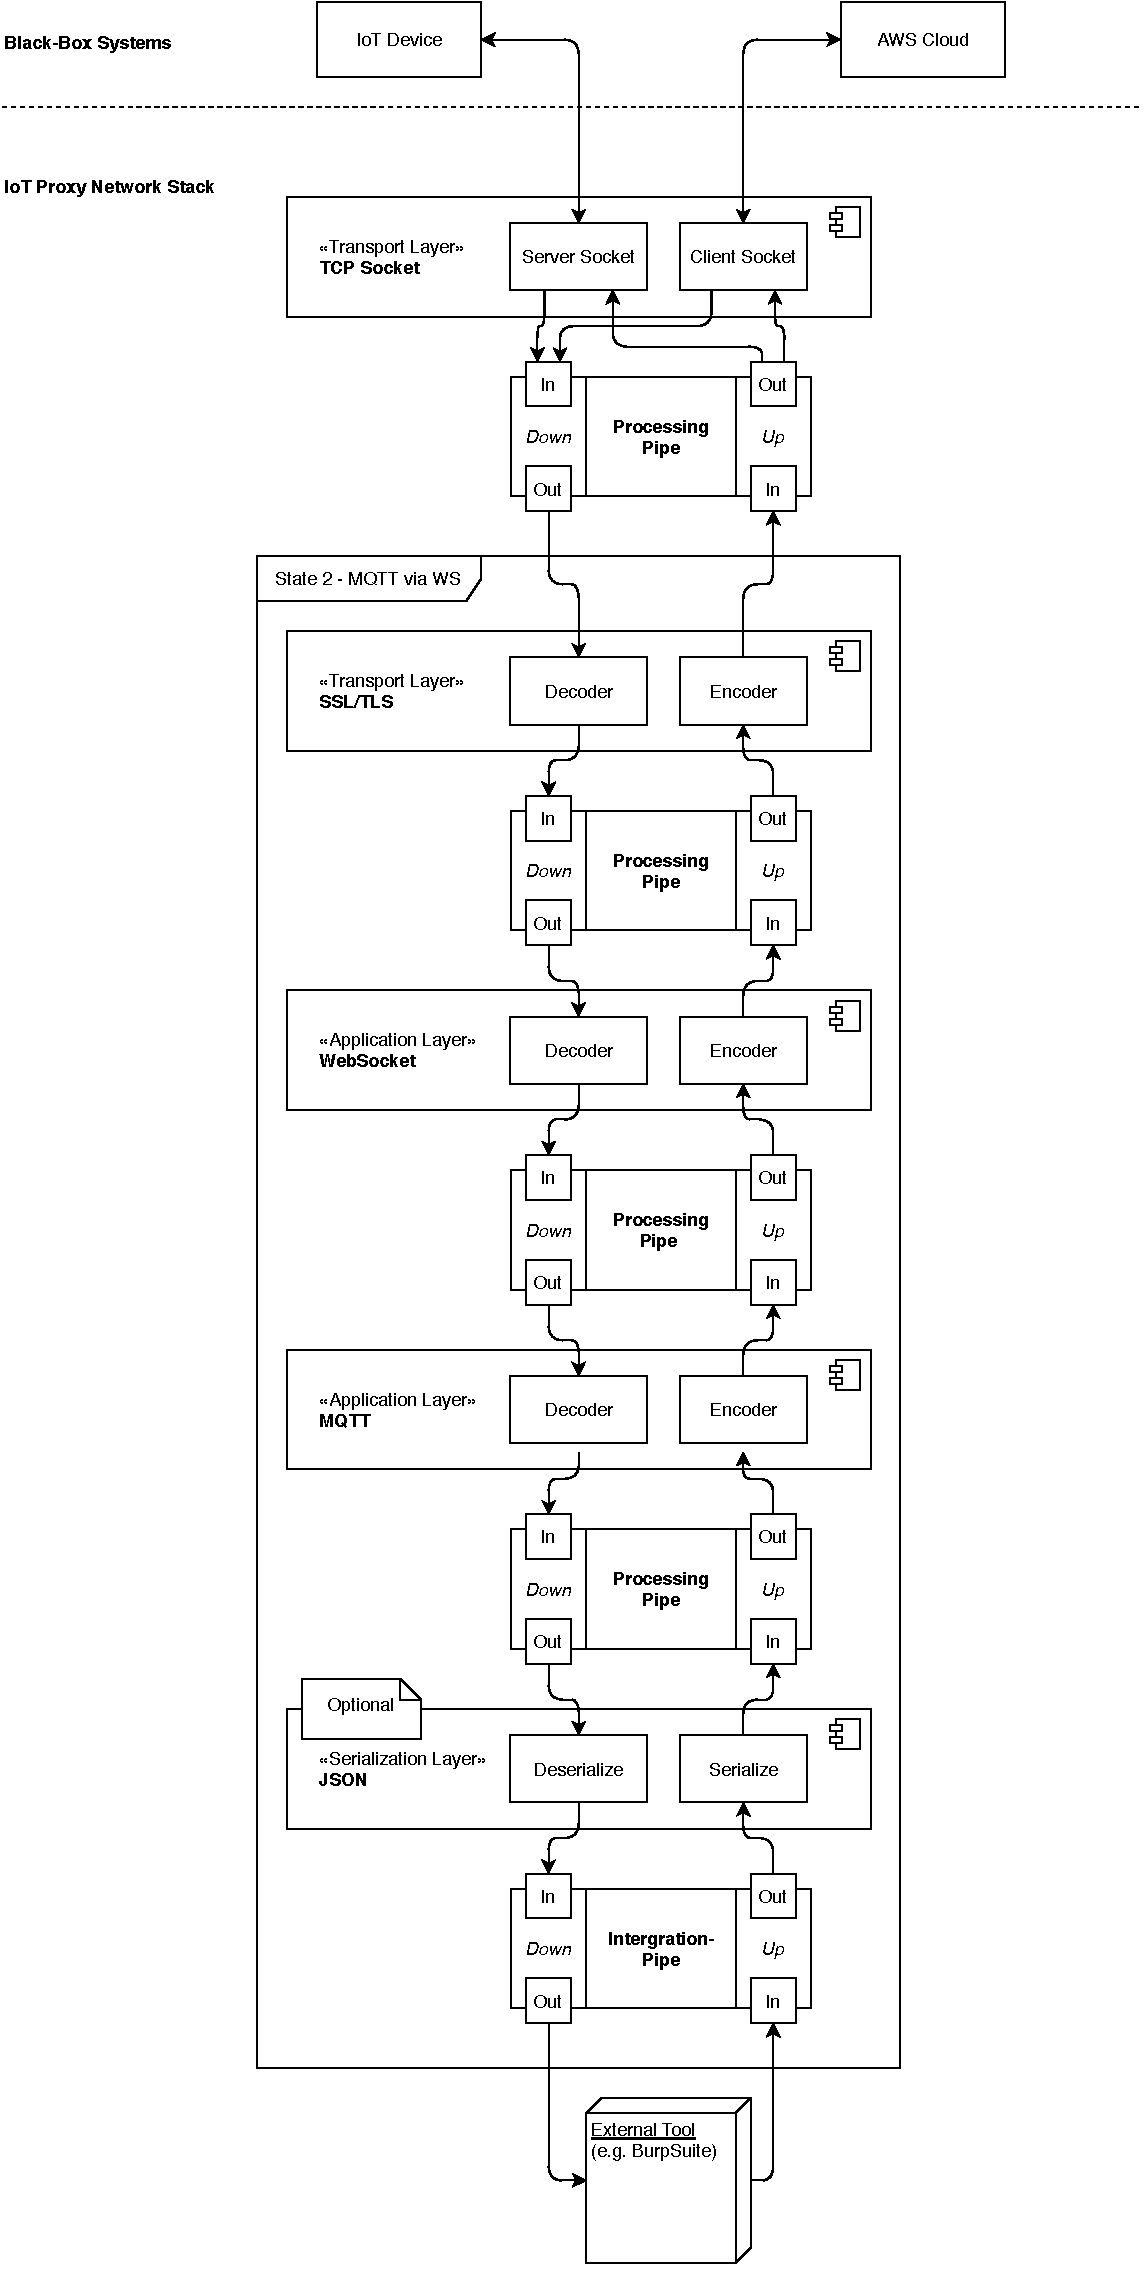
\includegraphics[width=10cm]{img/ch04/Architecture - PipesFilters 2.pdf}
    \captionof{figure}{\ac{AWS} \ac{IoT} Scenario - State 2: \ac{MQTT} via \ac{WS}}
    \label{fig:app-diag-pipesfilters-2}
\end{figure}
Once the prototype detects that the state must be changed to processing \ac{MQTT} over \ac{WS} communication, a different network stack is initialized and used, as shown in figure \ref{fig:app-diag-pipesfilters-2}. In this state, TLS-encryption is decrypted and passed into a \ac{WS} filter that (de-)serializes \ac{WS} packets. The payload of data frames is then forwarded to an \ac{MQTT} layer. In this specific configuration shown in figure \ref{fig:app-diag-pipesfilters-2}, the payload of \ac{MQTT} messages is (de-)serialized as \ac{JSON} before being sent to external tools by the integration pipe.

\subsection{Testing}
\label{sec:prototype-testing}
To test the prototype, a simple testbed was designed and implemented to realize scenario \#3 (discussed in section \ref{sec:example-scenarios}). It consisted of two Debian 10 machines that acted as a \ac{MQTT} broker and clients and a Kali Linux machine that ran the prototype and provided tools such as Wireshark that could be used for debugging and monitoring network traffic. All machines were connected to a single network (shown in figure \ref{fig:testbed-network}) and were assigned static \ac{IP} addresses. While this setup allowed for more sophisticated \ac{MITM} mechanisms such as \ac{ARP} spoofing, the decision was made to directly connect the \ac{MQTT} clients to the \emph{kali} machine to reduce complexity and accelerate and simplify testing. Separate machines were used for the \ac{MQTT} broker and clients so that actual \ac{MITM} attacks could be performed if the need to arose. Also, running the broker on a separate machine simplified debugging as network traffic could be attributed to broker or clients easier by examining the packets' source and destination \acp{IP}.\par

\begin{figure}[h]
    \centering
    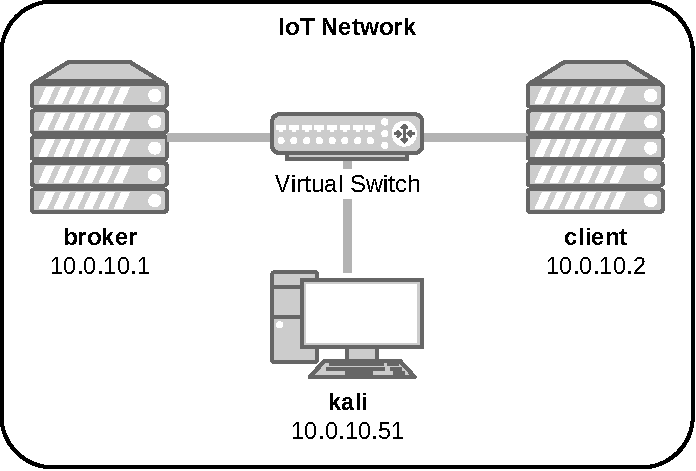
\includegraphics[width=8cm]{img/ch04/Testbed2.pdf}
    \captionof{figure}{A network diagram of the testbed that was used for testing the prototype.}
    \label{fig:testbed-network}
\end{figure}
The \ac{MQTT} broker software used on the \emph{broker} machine was Eclipse Mosquitto\footnote{https://mosquitto.org/} $1.5.7$ and had the \ac{WS} transport enabled to allow for clients to connect via \ac{WS}. The \ac{MQTT} clients running on the \emph{client} machine were implemented in Python using the Eclipse Paho library for Python (paho-mqtt\footnote{https://pypi.org/project/paho-mqtt/}).\par %TODO: Describe publish and processing pattern, ref mqtt graph below
\begin{figure}[h]
    \centering
    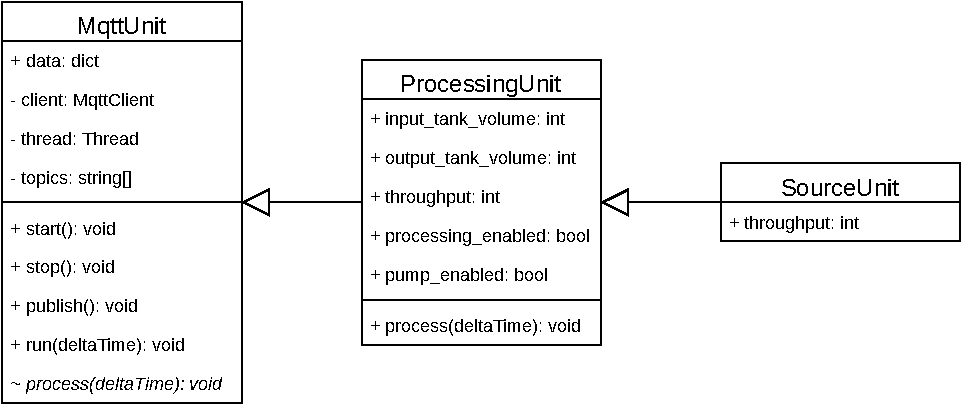
\includegraphics[width=14cm]{img/ch04/Testbed-Unit.pdf}
    \captionof{figure}{The \enquote{ProcessingUnit} data-structures represent individual stations of the simplified water treatment plant.}
    \label{fig:testbed-unit}
\end{figure}
The water treatment scenario required water treatment stations to be simulated individually as separate \ac{MQTT} clients, which was done by representing them as \enquote{ProcessingUnits} in the Python implementation of the testbed. As can be seen in figure \ref{fig:testbed-unit}, ProcessingUnits held individual \emph{MqttClient} instances running in separate threads, were subscribed to the topics of relevant other units such as their direct predecessors and successors and were capable of publishing their current state. Their \emph{process} method would be called cyclically and allow for units to calculate their intake, throughput and output.

\begin{figure}[h]
    \centering
    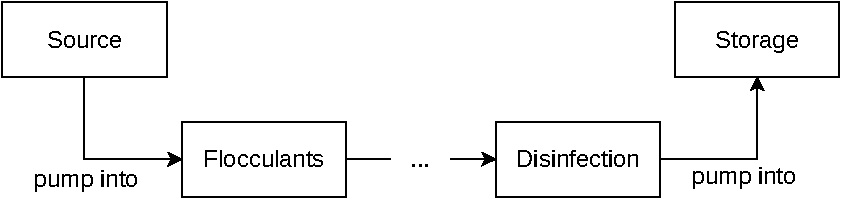
\includegraphics[width=12cm]{img/ch04/Testbed-Chain.pdf}
    \captionof{figure}{Chaining of the water treatment units, originating from a water source and eventually leading to a storage at the end of the processing pipeline.}
    \label{fig:testbed-chain}
\end{figure}
These units were then \enquote{chained} up (shown in figure \ref{fig:testbed-chain}) in the order in which they were presented in the scenario by specifying their direct predecessor and successor units: potentially contaminated water would be pumped out of the \emph{source}, processed by a series of stations and eventually flushed into the \emph{storage}. The \emph{source} was an instance of the \enquote{SourceUnit} that featured a throughput calculated by a sine-wave function that used the elapsed time since program startup as input parameter. Also, in order to keep the program running infinitely without either the \emph{source} \enquote{running dry} due to its input tank emptying or the \emph{storage} overfilling, the \emph{storage's} output was programmed to feed back into the \emph{source's} input tank (as can be seen in figure \ref{fig:mqtt-data}). While this was not a realistic approach, it kept the program's design simple and allowed for continuous testing and did not impact the \ac{MQTT} communication.

\begin{figure}[h]
    \centering
    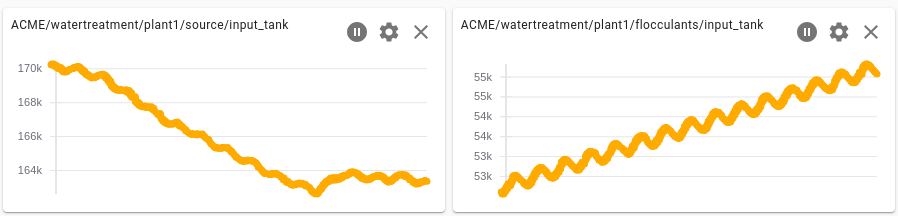
\includegraphics[width=14cm]{img/ch04/watertreatment-mqtt-short.png}
    \captionof{figure}{Screenshot of the application \enquote{MQTT Explorer} that was used to inspect and visualize the state of the water treatment plant. The left graph shows how the \emph{source's} input tank steadily emptied until it was filled by the \emph{storage's} output tank. The right graph shows how the \emph{flocculant} unit's input tank slowly filled up.} %TODO: Describe
    \label{fig:mqtt-data}
\end{figure}

\subsection{Implementation}
\label{sec:prototype-implementation}
The prototype was partially implemented over the course of ???%TODO: how many weeks?
weekly sprints after which work on the prototype was halted. It was written in TypeScript due to the language's flexibility and static typing. It allowed to precisely specify interfaces and its runtime (NodeJS) would allow it to make use of asynchronous programming, which would benefit this prototype. The rough design worked out in section \ref{sec:prototype-design} was specified in greater detail so individual classes could be derived and implemented.\par
\begin{figure}[h]
    \centering
    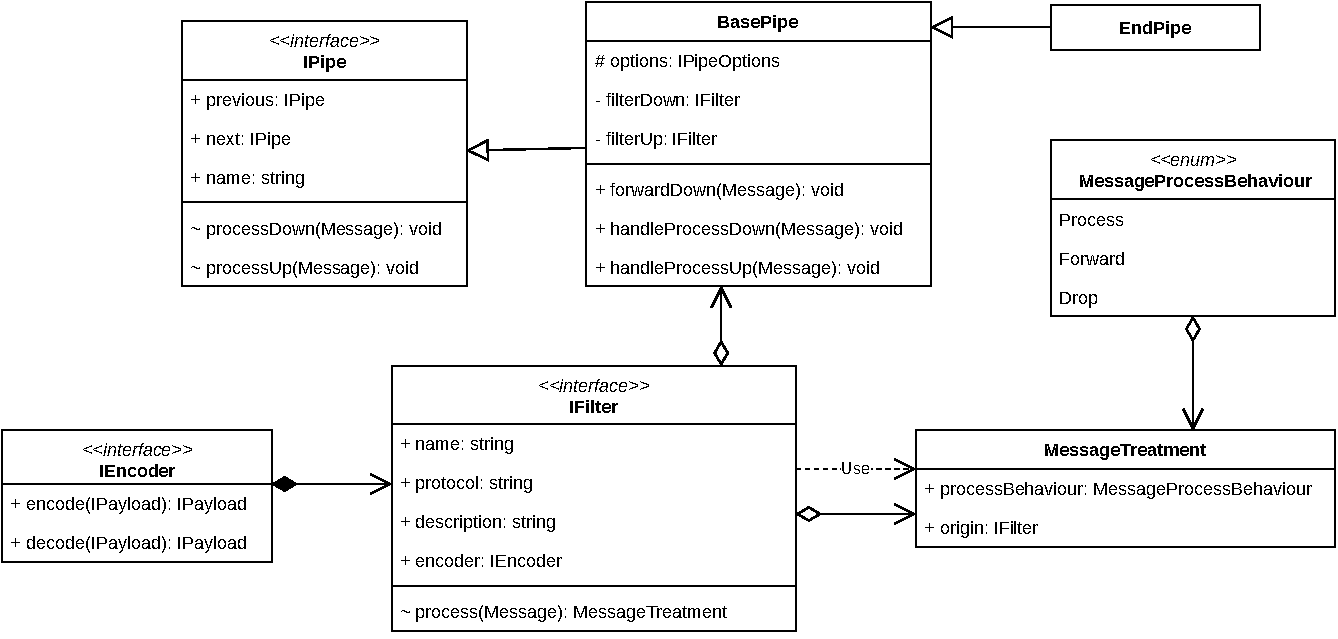
\includegraphics[width=14cm]{img/ch04/prototype/pipe-filter.pdf}
    \captionof{figure}{The classes and interfaces used to implement pipelines in the TypeScript prototype.}
    \label{fig:prototype-pipe-filter}
\end{figure}
\paragraph{Pipes and Filters} As shown in figure \ref{fig:prototype-pipe-filter} the pipeline design pattern was altered in such a way that the basic \emph{IPipe} interface was implemented by the \emph{BasePipe} class that held a reference to a single \emph{IFilter} but lacked a reference to an \emph{IEncoder}. Filters would hold a reference to encoders because encoders were used directly by filters for (de-)serialization prior to any other processing (such as executing scripts). Thus, encoders would not exist without filters, resulting in a composition relationship between the two. As indicated by their prefix \emph{IFilters} and \emph{IEncoders} were only interfaces that set a behaviour for their specific uses: encoders would implement (de-)serialization of specific protocols while filters added logic to processing (de-)serialized packets, such as executing scripts. The prototype implemented encoders for \ac{HTTP} and \ac{MQTT} as well as a \emph{BaseFilter} that did not add any logic to processing but allowed to test the encoder implementation. Also, specific \emph{NopFilter} and \emph{NopEncoder} (\enquote{Nop} meaning \enquote{no operation}) classes were implemented that did not implement any logic. This was used to test sending messages down and up the pipeline without processing them at all. The \ac{MQTT} encoder used the \enquote{mqtt-packet}\footnote{https://github.com/mqttjs/mqtt-packet, commit 4b6278d890e0c2fca01da62c5f9b63e05f5fd899} library which offered a comparatively simple API for serializing (\emph{generate(Packet)}) and de-serializing (\emph{parser.parse(Buffer)}). However, lacking a library that offered a similar low-level and simple API for \ac{HTTP} (de-)serialization, a custom encoder for these tasks was implemented. Due to \ac{HTTP} being a comparatively simple and text-based protocol, all that needed to be done for de-serialization was parsing the \ac{HTTP} headers (separated by new-lines) and, depending on whether or not the \enquote{Content-Length} header was present, extracting the \ac{HTTP} body.

\begin{figure}[h]
    \centering
    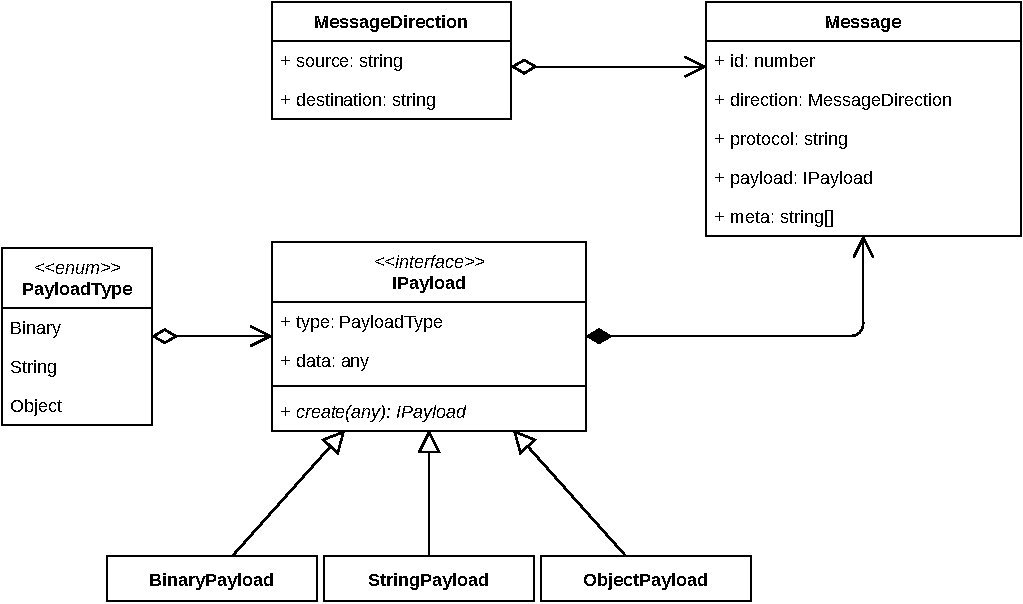
\includegraphics[width=14cm]{img/ch04/prototype/message-payload.pdf}
    \captionof{figure}{?} %TODO: Describe
    \label{fig:prototype-message-payload}
\end{figure}
\paragraph{Messages and Payloads}
The pipeline system implemented routing and processing of messages, however this required a concept of what messages are and how they convey the information required to perform meaningful and useful operations on network communication. Figure \ref{fig:prototype-message-payload} shows the classes and interfaces that defined the messages and payloads types. \emph{Messages} hold basic information such as a unique identifier, the communication protocol they were sent through and metadata that was used to store header information in. The \emph{IPayload} interface allowed for implementation and use of various payload formats such as raw binary information (e.g. \ac{MQTT} message bodies), string contents (e.g. \ac{HTTP} response bodies when the \emph{Content-Type} header indicated \emph{text} data) or JavaScript objects such as dictionaries that could hold arbitrary data for cases where there was no meaningful way to extract payloads from messages. The \emph{MessageDirection} structure was used to relay the message to the correct socket after it was processed by the pipeline.

\begin{figure}[h]
    \centering
    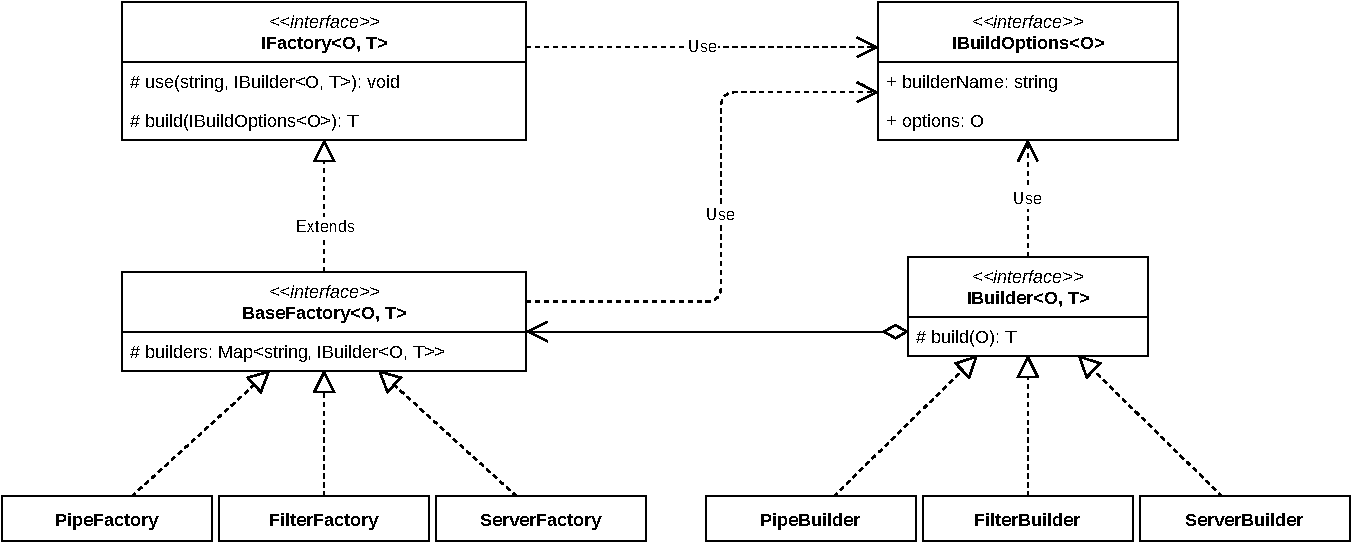
\includegraphics[width=14cm]{img/ch04/prototype/factory-builder.pdf}
    \captionof{figure}{?} %TODO: Describe
    \label{fig:prototype-factory-builder}
\end{figure}

\paragraph{Factories and Builders}
The requirement \enquote{F2 Network Stacks} implied a way of initializing various objects that represent pipelines, sockets and \acp{FSM}, dependent on configuration files loaded at runtime. As shown in figure \ref{fig:prototype-factory-builder}, the factory design pattern was used to provide an easy way to initialize pipes, filters, encoders and sockets while passing them metadata used for object creation. An \emph{IFactory} interface exposed simple methods for registering \emph{IBuilders} and building objects. The generic type parameters \emph{O} and \emph{T} were placeholders for type specific options (e.g. \emph{IPipeOptions} and \emph{IFilterOptions}) and the type of the created objects (e.g. \emph{IPipe} and \emph{IFilter}), respectively. The options types would contain information that was used for creating individual instances, such as a pipe's name or a server socket's address to listen on. The \emph{BaseFactory} class implemented the \emph{IFactory} interface and held an internal hash-map that was used to register \emph{IBuilders} by name. Lastly, the \emph{IBuilder} interface provided a method for initializing objects with the given options, providing default values for constructor parameters. There were static instances of factories and builders of pipes, filters and servers. For instance, the global server-factory \emph{SERVER\_FACTORY} used the global TCP server builder instance \emph{TCP\_SERVER\_BUILDER}.

%TODO: FSMs? Also, reference postmortem

\subsection{Insights Gained}
\label{sec:prototype-insights}
The following insights were gained through the prototypical implementation. Some resulted in questions relevant for the expert interviews that were to be held:
\begin{itemize}
    \item Due to the \ac{MTU}, large messages were broken into chunks that were transferred sequentially. This required the proxy to work on streams of incoming data and reassemble messages from said chunks. While individual \ac{MQTT} messages would often be short enough to be transmitted in a single \ac{TCP} packet, other communication protocols such as \ac{HTTP} could yield messages that were several hundred kilobytes or more in size (e.g. when downloading images). This also required the encoders to be stateful as they had to load data of incoming packets into individual buffers until they could parse complete messages, introducing the need to initialize one pipelines per device connected to the proxy application.
    \item Supporting multiple client devices was non-trivial as communication between clients and servers was not necessarily connection-oriented (e.g. \ac{HTTP} on the application level or \ac{UDP} on the transport level). \\
          \emph{Q1: Do penetration testers need to test multiple devices at the same time?}
    \item In some cases, e.g. with \ac{WS} data-frames, extending a message's payload resulted in its payload being split into multiple messages. This indirectly created new messages that, depending on the exact protocol used, needed to use generated values (such as an unique identifier) or context-specific information (e.g. authentication tokens used in \ac{HTTP} headers). Also, some libraries would generate those values themselves and not define ways to specify those manually.\\
          \emph{Q2: Do penetration testers require exact control over the implementation of protocols?}
    \item Manipulating messages, automatically via scripting or by hand using third-party integrations (e.g. to \emph{Burp Suite}), could introduce latency to the communication.\\
          \emph{Q3: Are there strict timing requirements during penetration tests?}
    \item Many libraries offered high-level functions to the programmer while avoiding exposure of low-level functionalities like crafting or parsing messages. Exposing such functionalities would require dissecting and altering libraries on a source-code level.
\end{itemize}

\section{Interviewing Experts for Insights}
\label{sec:interviews}
Interviews may be an efficient way to get an expert’s opinion on something they are proficient in. Thus, expert interviews were conducted to let security researchers give insight into their everyday work and the challenges they face when working with \ac{IoT} and \ac{IIoT} applications. The information and insights gathered in these interviews were then used to model a persona, various work scenarios and use-cases that as a whole aim to represent their work.

\subsection{Interview Guideline}
An interview guideline (shown in \emph{TBD}) %TODO: Reference appended interviews + guideline
was created to keep focus on key points during interviews so that interviewees would not stray too far from the relevant points. The guideline also served as a checklist so the interviewer could make sure that all questions and points that should be covered  initially, were in fact covered by the end of the interviews. It was composed of three sections:

\paragraph{1. Experiences with IoT} The answers to these questions would give insights into what kind of applications the security researchers had worked on in the past. Answers to question \emph{1.1.} were of particular interest as they might represent what technologies were being examined by security researchers and may be popular in today’s applications.
\paragraph{2. Processes in Everyday Life} This section aimed to cover questions about the processes and tasks security researchers perform during penetration tests of IoT applications in their everyday life. Ideally, answers to those questions would show the approaches taken and challenges faced during their work, uncovering potential needs and underlying motivation.
\paragraph{3. The Future of IoT} This section had security researchers assess what the future of IoT may be like from their point of view. This required the interviewees to make a critical assessment of the status quo.


\subsection{Conducting Interviews}
Interviews were conducted with six
\emph{NVISO} employees (Patrick Eisenschmidt, Cédric Bassem, Théo Rigas, Oliver Nettinger, Pierre-Alain Mouy, Jonah Bellemans) that all had worked on security assignments on \ac{IoT} or \ac{IIoT} applications in the past. There is considerable variety in
\begin{itemize}
    \item the experience they had in working on security assignments in general: all interviewees had a strong background in cyber security that reached back multiple years except one who was a working student at \emph{NVISO Labs} (Bellemans).
    \item the experience they have had in working on \ac{IoT}/\ac{IIoT} applications: two interviewees worked on assessing \ac{IoT}/\ac{IIoT} applications only occasionally (Eisenschmidt, Mouy), one was part of a car manufacturer's automotive security team in the past (Nettinger) and two were part of \emph{NVISO Labs} and worked with smart devices on a regular basis (Bassem, Rigas).
    \item the focus of their everyday work: two interviewees were \emph{NVISO} chief executives and switched to working on management tasks rather than security assessments (Nettinger, Mouy), one was a working student finishing their master's thesis with a focus on legal aspects of \ac{IoT} devices (Bellemans) and the remaining three worked on security assessments in a variety of fields (Eisenschmidt, Bassem, Rigas).
\end{itemize}
The duration of the interviews varied from 45 minutes to two hours depending on the amount and level of detail of information provided by the interviewees and the number of times that the interviewer had to ask further questions.\par
Due to the COVID-19 pandemic, interviews were conducted remotely over Microsoft Teams and recorded for later review and analysis. All interviews were conducted successfully, however some problems were had: due to unstable internet connections interviews were sometimes interrupted for up to 30 seconds, low bandwidth and low microphone quality sometimes made making out specific words and phrases very hard.

\subsection{Interview Analysis}
The answers interviewees gave to the various questions present in the interview guide varied greatly in detail. The following paragraphs attempt to summarize the essential statements interviewees made, sorted by the sections of the interview guide and ending with conclusions drawn from the interviews.

\paragraph{1. Experiences with \ac{IoT}} Asked about the technologies they encountered in their work, most interviewees stated that \ac{MQTT} (5/6) and \ac{HTTP} (6/6) were widely used in the smart applications they assessed. For \ac{IoT} devices they found that Espressif microcontrollers such as the ESP32 and ESP8266 were used (2/6). Especially in cheap devices they found that custom protocols and infrastructure were used (2/6), whereas high-end devices usually used \ac{MQTT} and \ac{HTTP} and worked with well-known cloud infrastructures such as \ac{AWS}, Microsoft Azure or Google Cloud Platform. Most interviewees worked on Smart Home products (4/6) with one notable exception being Nettinger who worked on Smart Cars.\\
Usually, there were no technical constraints for the interviewees when performing security assessments. There were some non-technical constraints such as working from a black-box perspective rather than working from a white-box perspective that would allow evaluating more security aspects of a system in less time (Eisenschmidt, Bassem, Rigas). Depending on the client and the exact application that was to be tested, interviewees said that they made use of either mobile lab environments (2/6) or stationary lab environments (3/6). Also, interviewees stated that they usually assessed devices and applications individually.%Single devices?

\paragraph{2. Processes in Everyday Life} Regarding the goals of their assessments, interviewees would take on one of two approaches: The first was penetration testing (Eisenschmidt, Bassem, Rigas), aiming to evaluate as many components of a system as they could during their assessment. The second was red-teaming (Nettinger, Mouy, Bassem, Rigas) which aimed to get some level of access, preferably privileged, to a device or server in order to take influence on the application's logic or exfiltrate data. The scopes of their assessments was usually defined by the client and could include testing of devices, applications and firmware or performing source-code and cloud configuration reviews (Eisenschmidt).\\
The high-level tasks carried out during assessments would generally be the same across assessments: first, interviewees would inspect applications passively from a black-box perspective without interacting with them. This could incorporate looking for hardware interfaces on a device (Bassem, Rigas), looking for open network ports (Bellemans), reverse engineering Android applications and inspecting certain artefacts as manifest files (Eisenschmidt) and monitoring applications' network traffic (Bellemans). Nettinger stated that when working with cars, fuzzing was a task often carried out against bus protocol implementations because the devices implementing those protocols were often supplied by third parties and source-code was usually not available.\\
The tools used by the interviewees were mostly dependent on the technologies and protocols they worked with, such as Burp Suite for examining \ac{HTTP} communication (Eisenschmidt, Bassem, Rigas, Nettinger, Mouy, Bellemans). However, some general tools were used for information gathering (nmap and nessus), monitoring (Wireshark) and networking (socat, mitmproxy). Bassem, Rigas and Mouy stated that they would occasionally implement their own tools or scripts when they found that there either were no tools available that suited their needs or those tools would not work. According to Rigas, tools were highly specific to custom setups and preparing them up for use could be more challenging than actually using them. Bassem, Rigas and Bellemans stated that tools were often immature. Speaking of their automated tests performed on smart devices Bellemans criticized that automated tools often yielded inaccurate or incorrect results such as nmap reporting a game-server running on a smart lightbulb. Also, when manipulating communication of applications, interviewees generally were not interested in manipulating metadata such as headers but focused on the messages' payloads.

\paragraph{3. The Future of \ac{IoT}} When asked about the current challenges the interviewees were facing working on \ac{IoT} assessments, they gave very individual answers: Eisenschmidt expressed concerns about data protection and cloud environments being a rather new technology that requires engineers to securely configure them. Mouy and Eisenschmidt stated that protocols and frameworks became increasingly complex and more and more devices interacted with each other, adding complexity to the security assessments. Also, there were a lot of custom protocols and frameworks that lacked proper tooling and were time-consuming to asses (Bellemans, Mouy). When working on \ac{IoT} assignments, clients often had a traditional view on the assignments and occasionally wanted the testers to perform black-box tests only although additional white-box tests would potentially help covering more components and internals of applications (Bassem, Rigas).\\
Half of the interviewees stated that cloud computing will be more important and present in the future (Eisenschmidt, Nettinger, Mouy). They expect continued use of the comparatively old but proven \ac{HTTP} (Bassem, Rigas) and the well-accepted \ac{MQTT} (Bassem, Rigas, Nettinger). Regarding software development, they expect manufacturers of smart systems to involve IT security more into their development process (Bassem, Rigas, Nettinger) as well as use standardized frameworks (Mouy, Bassem, Rigas). However, they also stated concerns about the growing complexity of frameworks and the uncertainty of which frameworks will eventually gain wide acceptance (Bassem, Rigas). Regarding autonomous driving, Nettinger noted that current discussions about legal topics (such as the question about which party is to  assume liability in case of accidents) will likely not come to an end anytime soon. Concerned about security and safety aspects of future \ac{IoT} applications, Bellemans expressed the need for smart applications to be labelled or certified and they referred to the European cybersecurity certification framework that is being worked on by the \ac{ENISA}.


\paragraph{Conclusions}
%TODO: Answer questions from 4.1.6
The interviews yielded a set of both very interesting and relevant insights into the interviewees' work and fields of expertise. The following insights served as a guide for further development of the proxy application:
\begin{itemize}
    \item Smart devices often communicated via \ac{HTTP} and \ac{MQTT}. While the tools for security assessments with \ac{HTTP} were very mature, there was a perceived lack of tools for \ac{MQTT}.
    \item Often times, smart applications made use of proprietary protocols and infrastructure. While this was a fact the interviewees expect to be of less significance in the future, it still was of greater significance then.
    \item Penetration testers usually did not intend to test the protocol implementations used by applications but the contents transmitted over these protocols.
    \item Tools for working with specific protocols were often very immature and both installation and usage involved a lot of work.
\end{itemize}
Also, the questions raised in section \ref{sec:prototype-insights} were answered and could be used to derive assumptions to take into account when creating a software design for a proxy application:
\begin{enumerate} %TODO: Cite interviewees!
    \item [\textbf{Q1}] The interviewees usually tested individual devices one at a time.
          Therefore, an assumption can be made that the software design should not aim for testing multiple devices at once.
    \item [\textbf{Q2}] Interviewees stated that during tests there is a strong focus on the message payloads. They do not test protocol implementations and usually do not have to manipulate protocol headers. Thus, the software design should aim to provide penetration testers with access to message payloads rather than protocol headers.
    \item [\textbf{Q3}] According to the interviewees, they did not encounter strict timing requirements such as real-time communication during their assessments. As a result, the software design should not take timing into account any may envision mechanisms that potentially introduce latency (such as queueing messages).
\end{enumerate}
%Q1: Do penetration testers need to test multiple devices at the same time?
%Q2: Do penetration testers require exact control over the implementation of protocols?
%Q3: Are there strict timing requirements during penetration tests?
These insights were translated into the following, new non-functional requirements:

\begin{center}
    \begin{tabular}{|p{1cm}|p{12cm}|}
        \hline
        \textbf{N4} & \textbf{Extensibility}                                                                                                                      \\ \hline
        \multicolumn{2}{|p{12cm}|}{To allow for future implementation of further communication protocols the software shall be implemented in a modular fashion.} \\ \hline
    \end{tabular}
\end{center}
\begin{center}
    \begin{tabular}{|p{1cm}|p{12cm}|}
        \hline
        \textbf{N5} & \textbf{Deployment}                                                                                                                                                           \\ \hline
        \multicolumn{2}{|p{12cm}|}{To allow the proxy application to be installed and used in a repeatable and reliable way, the proxy application shall be distributed using a deployment system.} \\ \hline
    \end{tabular}
\end{center}

\section{Analysis of Existing Software}
\label{sec:analysis-existing-software}
\emph{TBD: Explain why the tools shown in 3 are not up for the task}

\begin{table}[h]
    \centering
    \begin{tabular}{r|c|c|c|c|c|c}
        \toprule
        \thead{$Name$} & \thead{$Latest$                                                                                                    \\$Release$} & \thead{$Implemented$\\$in$} & \thead{$Supported$\\$Protocols$} & \thead{$R$} & \thead{$W$} & \thead{$D$}\\
        \midrule
        Wireshark      & 2020-07-01        & C      & Various    & \cellcolor{green!25}F  & \cellcolor{red!25}N    & \cellcolor{red!25}N    \\
        \midrule
        MITMf          & 2015-08-28        & Python & Various    & \cellcolor{green!25}F  & \cellcolor{green!25}F  & \cellcolor{green!25}F  \\ %https://github.com/byt3bl33d3r/MITMf
        \midrule
        Ettercap       & 2019-07-01        & C      & Various    & \cellcolor{green!25}F  & \cellcolor{green!25}F  & \cellcolor{green!25}F  \\
        \midrule
        bettercap      & 2020-03-13        & Go     & Various    & \cellcolor{green!25}F  & \cellcolor{green!25}F  & \cellcolor{green!25}F  \\
        \midrule
        mitmproxy      & 2020-03-13        & Python & HTTP/S, WS & \cellcolor{orange!25}P & \cellcolor{orange!25}P & \cellcolor{orange!25}P \\ %https://github.com/mitmproxy/mitmproxy
        \midrule
        mProxy         & Pre-Releases only & Go     & MQTT       & ?                      & \cellcolor{green!25}F  & -                      \\ %https://github.com/mainflux/mproxy
        \midrule
        IOXY           & Source only       & Go     & MQTT       & \cellcolor{green!25}F  & \cellcolor{green!25}F  & \cellcolor{green!25}F  \\ %https://github.com/mainflux/mproxy
        \bottomrule
    \end{tabular}
    \caption[Comparison of existing software]{Comparison of existing software where $R$, $W$ and $D$ describe read, write and deletion capabilities, respectively. $F$, $N$ and $P$ indicate full, no or partial functionality, respectively.}
    \label{table:comparison-existing-software}
\end{table}